\documentclass{ustb-thesis}

% \syntaxonly

\usepackage{graphicx}

% 论文基本信息
\newcommand{\ctitlefirst}{基于模糊测试的RISC-V}  % 中文标题第一行
\newcommand{\ctitlesecond}{SBI系统测试框架研究}  % 中文标题第二行
\newcommand{\etitlefirst}{A Research Based on XXXXX}  % 英文标题第一行
\newcommand{\etitlesecond}{XXXX System Research}  % 英文标题第二行
\newcommand{\collage}{计算机与通信工程学院}  % 学院
\newcommand{\class}{物联212}  % 班级
\newcommand{\name}{王诺贤}  % 作者
\newcommand{\id}{U202141934}  % 学号
\newcommand{\firstmentorname}{XXX}  % 第一指导老师姓名
\newcommand{\firstmentortitle}{教授}  % 第一指导老师职称
\newcommand{\scondmentorname}{XXX}  % 第二指导老师姓名
\newcommand{\scondmentortitle}{副教授}  % 第二指导老师职称
\renewcommand{\year}{2025}  % 年份
\renewcommand{\month}{05}  % 月份
\newcommand{\miji}{公开}  % 密级
\newcommand{\ckeywords}{模糊测试, RISC-V, SBI}  % 中文关键词
\newcommand{\ekeywords}{Fuzzing, RISC-V, SBI}  % 英文关键词


\begin{document}
\pagenumbering{gobble}
\begin{titlepage}
  \noindent
\includegraphics[width=0.48\textwidth]{imgs/logo.png}

  \begin{flushright}
    {\songti\zihao{5}密级:\uline{\makebox[2cm][c]{公开}}}
  \end{flushright}

  \vspace{3cm}

  {\noindent\heiti\zihao{-0}本科生毕业设计(论文)}

  \vspace{4.5cm}

  \zihao{-3}

  {\heiti 题\hspace{0.5em}目:}\uline{\makebox[7.5cm][c]{\ctitlefirst}}

  \vspace{0.4cm}

  {\heiti \hspace{3.5em}}\uline{\makebox[7.5cm][c]{\ctitlesecond}}

  \vspace{0.4cm}

  {\heiti 作\hspace{0.5em}者:}\uline{\makebox[7.5cm][c]{\name}}

  \vspace{0.4cm}

  {\heiti 学\hspace{0.5em}号:}\uline{\makebox[7.5cm][c]{\id}}

  \vspace{0.4cm}

  {\heiti 学\hspace{0.5em}院:}\uline{\makebox[7.5cm][c]{\collage}}

  \vspace{0.4cm}

  {\heiti 专\hspace{0.5em}业:}\uline{\makebox[7.5cm][c]{\major}}

  \vspace{0.4cm}

  {\heiti 成\hspace{0.5em}绩:}\uline{\makebox[7.5cm][c]{}}

  \vspace{0.7cm}

  \begin{center}
    {\songti\zihao{4}\year\ 年\ \month\ 月}
  \end{center}

\end{titlepage} 

\cleardoublepage

\begin{titlepage}
  
\begin{tikzpicture}[remember picture, overlay]
  % ---- 1. 绘制双线边框 ----
  \draw[double, line width=1pt, double distance=1pt]
      ($(current page.north west)+(3cm,-3cm)$) rectangle 
      ($(current page.south east)+(-1cm,3cm)$);

  % ---- 2. 在指定位置插入文字 ----
  \node at ($(current page.center)+(1cm,6.5cm)$) {
\includegraphics{imgs/title.pdf}};
  \node[align=center, font=\heiti\zihao{-3}\bfseries\selectfont] 
      at ($(current page.center)+(1.5cm,2cm)$) {
        题\hspace{2em}目:\songti\mdseries\uline{\makebox[7cm]{\ctitlefirst}}
      };
  \node[align=center, font=\heiti\zihao{-3}\bfseries\selectfont] 
      at ($(current page.center)+(1.5cm,0.7 0cm)$) {
        \hspace{5em}\songti\mdseries\uline{\makebox[7cm]{\ctitlesecond}}
      };
  \node[align=center, font=\heiti\zihao{-3}\bfseries\selectfont] 
      at ($(current page.center)+(1.5cm,-0.6cm)$) {
        英文题目:\songti\mdseries\uline{\makebox[7cm]{\etitlefirst}}
      };
  \node[align=center, font=\heiti\zihao{-3}\bfseries\selectfont] 
      at ($(current page.center)+(1.5cm,-1.9cm)$) {
        \hspace{5em}\songti\mdseries\uline{\makebox[7cm]{\etitlesecond}}
      };
  \node[align=center, font=\heiti\zihao{-3}\bfseries\selectfont] 
      at ($(current page.center)+(1.5cm,-3.2cm)$) {
        学\hspace{2em}院:\songti\mdseries\uline{\makebox[7cm]{\collage}}
      };
  \node[align=center, font=\heiti\zihao{-3}\bfseries\selectfont] 
      at ($(current page.center)+(1.5cm,-4.5cm)$) {
        班\hspace{2em}级:\songti\mdseries\uline{\makebox[7cm]{\class}}
      };
  \node[align=center, font=\heiti\zihao{-3}\bfseries\selectfont] 
      at ($(current page.center)+(1.5cm,-5.8cm)$) {
        学\hspace{2em}生:\songti\mdseries\uline{\makebox[7cm]{\name}}
      };
  \node[align=center, font=\heiti\zihao{-3}\bfseries\selectfont] 
      at ($(current page.center)+(1.5cm,-7.1cm)$) {
        学\hspace{2em}号:\songti\mdseries\uline{\makebox[7cm]{\id}}
      };
  \node[align=center, font=\heiti\zihao{-3}\bfseries\selectfont] 
      at ($(current page.center)+(1.5cm,-8.4cm)$) {
        指导教师:\songti\mdseries\uline{\makebox[2.6cm]{\firstmentorname}}
        \heiti\bfseries 职称:\songti\mdseries\uline{\makebox[2.65cm]{\firstmentortitle}}
      };
  \node[align=center, font=\heiti\zihao{-3}\bfseries\selectfont] 
      at ($(current page.center)+(1.5cm,-9.7cm)$) {
        指导教师:\songti\mdseries\uline{\makebox[2.6cm]{\secondmentorname}}
        \heiti\bfseries 职称:\songti\mdseries\uline{\makebox[2.65cm]{\secondmentortitle}}
      };

\end{tikzpicture}
\end{titlepage} 

\cleardoublepage


{\centering\chapter*{声\hspace{2em}明}}
{
  \songti\zihao{4}\linespread{2.1}\selectfont
  本人郑重声明:所呈交的论文是本人在指导教师的指导下进行的研究工作及取得研究结果。论文在引用他人已经发表或撰写的研究成果时,已经作了明确的标识;除此之外,论文中不包括其他人已经发表或撰写的研究成果,均为独立完成。其他同志对本文所做的任何贡献均已在论文中做了明确的说明并表达了谢意。\par

  \vspace{4.5cm}

  \begin{flushright}
  
  学生签名:\uline{\makebox[3cm]{}}\hspace{1.5em}\uline{\makebox[4em]{}}年\uline{\makebox[1.5em]{}}月\uline{\makebox[1.5em]{}}日

  \vspace{2cm}

  导师签名:\uline{\makebox[3cm]{}}\hspace{1.5em}\uline{\makebox[4em]{}}年\uline{\makebox[1.5em]{}}月\uline{\makebox[1.5em]{}}日

  \end{flushright}
}

\cleardoublepage

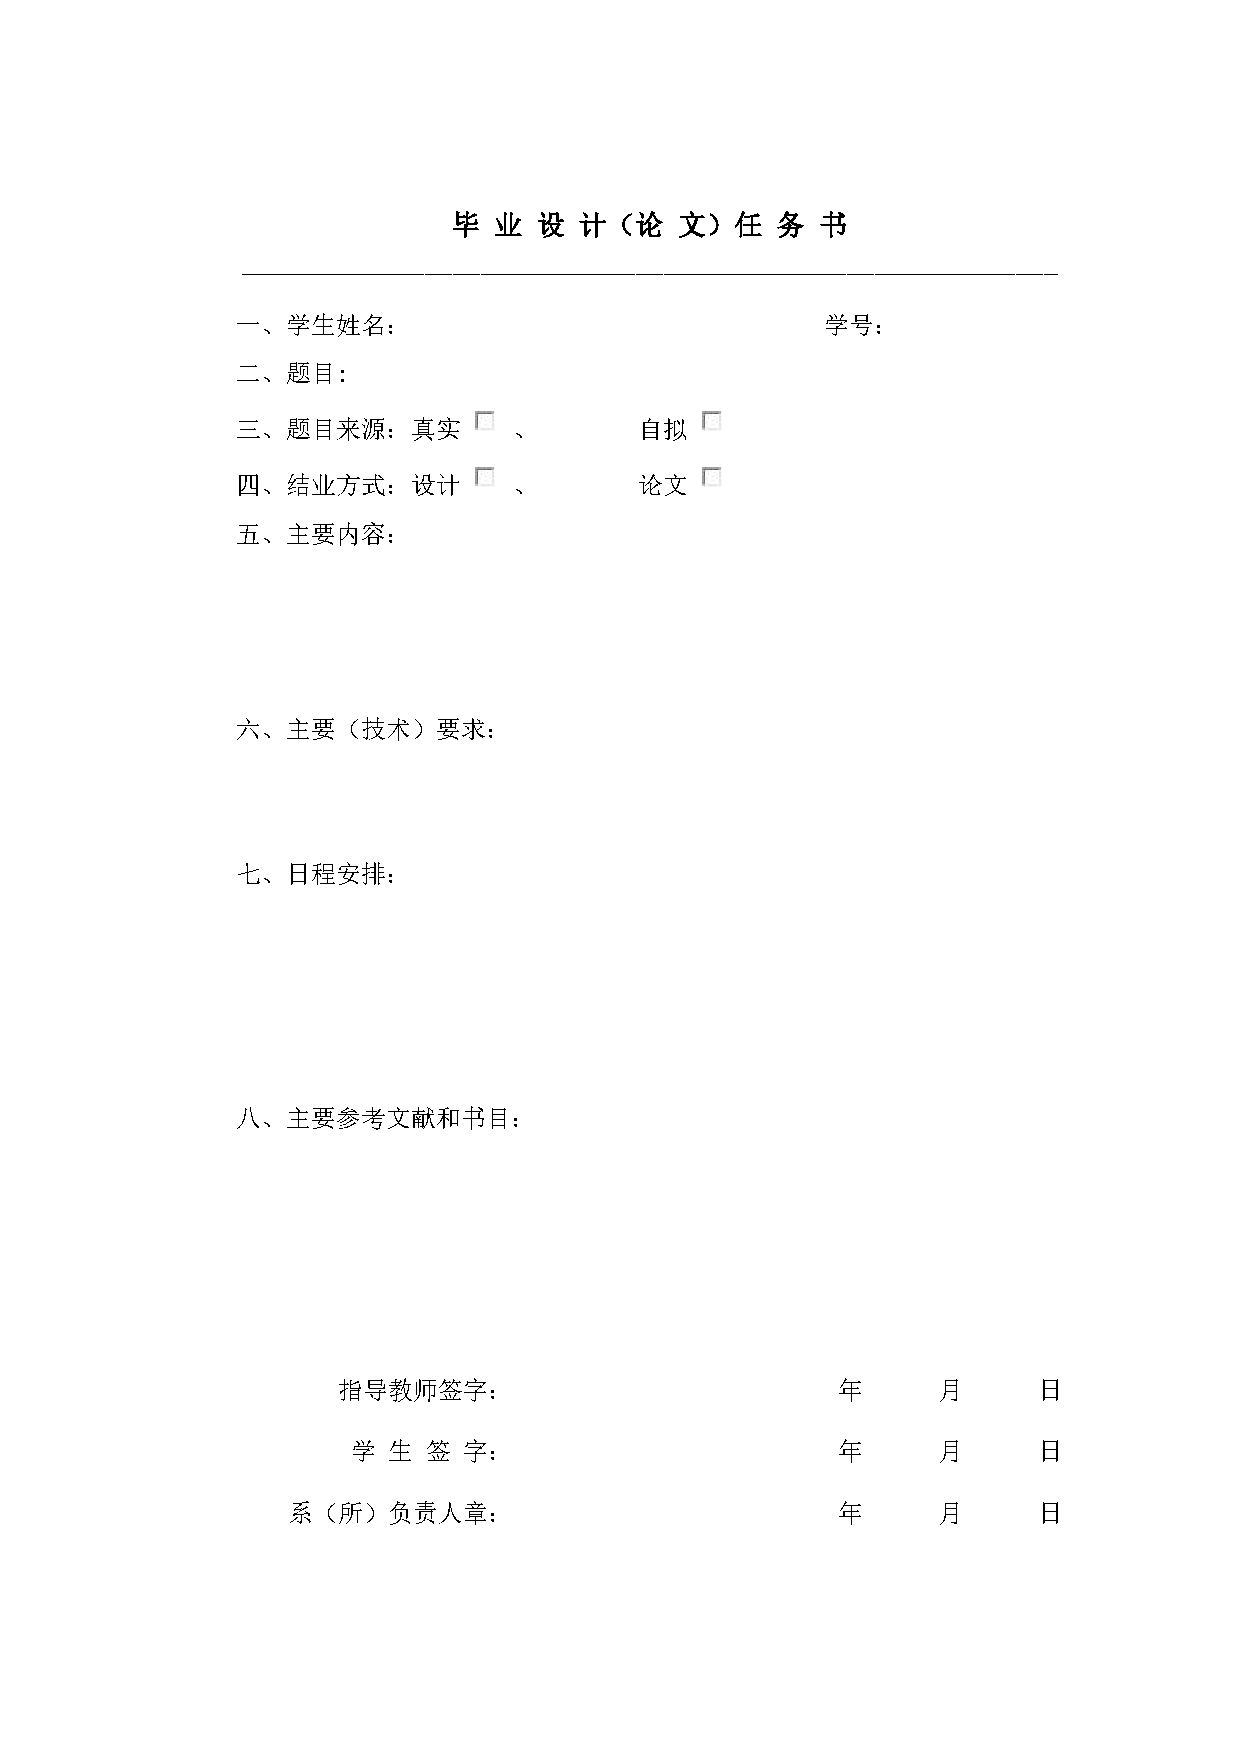
\includepdf[pages=-]{src/4-taskplan.pdf}

\cleardoublepage

\pagenumbering{Roman}

\addcontentsline{toc}{chapter}{摘\hspace{1em}要}


{\centering\chapter*{摘\hspace{1em}要}}

% 中文摘要

这是一段很长很长很长很长很长很长很长很长很长很长很长很长很长很长很长很长很长很长很长很长很长很长很长很长很长很长很长很长很长很长很长很长很长很长很长很长很长很长很长很长很长很长很长很长很长很长很长很长很长很长很长很长很长很长很长很长很长很长很长很长很长很长很长很长很长很长很长很长很长很长很长很长很长很长很长很长很长很长很长很长很长很长很长很长很长很长很长很长很长很长很长很长很长很长很长很长很长很长很长很长很长很长很长很长很长很长很长很长很长很长很长很长很长很长很长很长很长很长很长很长很长很长很长很长很长很长很长很长很长很长很长很长很长很长很长很长很长很长很长很长很长很长很长很长很长很长很长很长很长很长很长很长很长很长很长很长很长很长很长很长很长很长很长很长很长很长很长很长很长很长很长很长很长很长很长很长很长很长很长很长很长很长很长很长很长很长很长很长很长很长很长很长很长很长很长很长很长很长很长很长很长很长很长很长很长很长很长很长很长很长很长很长很长很长很长很长很长很长很长很长很长很长很长很长很长很长很长很长很长很长很长很长很长很长很长很长很长很长很长很长很长很长很长很长很长很长很长很长很长很长很长很长很长很长很长很长很长很长很长很长很长很长很长很长很长很长很长很长很长很长很长很长很长很长很长很长很长很长很长很长很长很长很长很长很长很长很长很长很长很长很长很长很长很长很长很长很长很长很长很长很长很长很长很长很长很长很长很长很长很长很长很长很长很长很长很长很长很长很长很长很长很长很长很长很长很长很长很长很长很长很长很长很长很长很长很长很长很长很长很长很长很长很长很长很长很长很长很长很长很长很长很长很长很长很长很长很长很长很长很长很长很长很长很长很长很长很长很长很长很长很长很长很长很长很长很长很长很长很长很长很长很长很长很长很长很长很长很长很长很长很长很长很长很长很长很长很长很长很长很长很长很长很长很长很长很长很长很长很长很长很长很长很长很长很长很长很长很长很长很长很长很长很长很长很长很长很长很长很长很长很长很长很长很长很长很长很长很长很长很长很长很长很长很长很长很长很长很长很长很长很长很长很长很长很长很长很长很长很长很长很长很长很长很长很长很长很长很长很长很长很长很长很长很长很长很长很长很长很长很长很长很长很长很长很长很长很长很长很长很长很长很长很长很长很长很长很长很长很长很长很长很长很长很长很长很长很长很长很长很长很长很长很长很长很长很长很长很长很长很长很长很长很长很长很长很长很长很长很长很长很长很长很长很长很长很长很长很长很长很长很长很长很长很长很长很长很长很长很长很长很长很长很长很长很长很长很长很长很长很长很长很长很长很长很长很长很长很长很长很长很长很长很长很长很长很长很长很长很长很长很长很长很长很长很长很长很长很长很长很长很长很长很长很长很长很长很长很长很长很长很长很长很长很长很长很长很长很长很长很长很长很长很长很长很长很长很长很长很长很长很长很长很长很长很长很长很长很长很长很长很长很长很长很长很长很长很长很长很长很长很长很长很长很长很长很长很长很长很长很长很长很长很长很长很长很长很长很长很长很长很长很长很长很长很长很长很长很长很长很长很长很长很长很长很长很长很长很长很长很长很长很长很长很长很长很长很长很长很长很长很长很长很长很长很长很长很长很长很长很长很长的文字。

\vfill

{
  \heiti\zihao{-4}\bfseries 关键词:\ckeywords
}

\vspace{3cm}

\cleardoublepage

\addcontentsline{toc}{chapter}{Abstract}

{\centering\chapter*{\etitlefirst\ \etitlesecond}}

{\centering\heiti\zihao{-3}\selectfont\bfseries Abstract\par}

\vspace{27pt}

% 英文摘要

This is a very very very very very very very very very very very very very very very very very very very very very very very very very very very very very very very very very very very very very very very very very very very very very very very very very very very very very very very very very very very very very very very very very very very very very very very very very very very very very very very very very very very very very very very very very very very very very very very very paragraph.

\vfill

{
  \heiti\zihao{-4}\bfseries Keywords: \ekeywords
}

\vspace{3cm}


\cleardoublepage

\tableofcontents

\cleardoublepage

\addcontentsline{toc}{chapter}{插图或附表清单}  % 将当前页面添加到目录中
{\centering\chapter*{插图或附表清单}}  % 页面标题
% 注意:修改该页面标题时请将上面两行内部内容一起修改

插图或附表清单并非必要。论文中如图表较多,可以有此页。图的清单应有图号、图题名和页码。表的清单应有表号、表题名和页码。

根据所列内容,可将本页标题分别更改为“插图清单”、“附表清单”。

此页并非必要,\textbf{不用此页时请删除}。  % 插图或附表清单页面,不需要时请删除此行

\cleardoublepage

\addcontentsline{toc}{chapter}{注释说明清单}  % 将当前页面添加到目录中
{\centering\chapter*{注释说明清单}}  % 页面标题
% 注意:修改该页面标题时请将上面两行内部内容一起修改

此页并非必要。符号、标志、缩略词、首字母缩写、计量单位等的注释说明,如需汇集,可集中置于此页。 

根据所列内容,将本页标题分别更改为“符号清单”、“标志清单”、“缩写清单”、“计量单位清单”等。 

此页并非必要,\textbf{不用此页时请删除}。  % 注释说明清单页面,不需要时请删除此行

\cleardoublepage

\pagenumbering{arabic}

% 正文页面,删除添加章节请修改这里的内容

\chapter{引\hspace{1em}言}

引言简要说明研究工作的目的、范围、相关领域的前人工作和知识空白、理论基础和分析、研究设想、研究方法和实验设计、预期结果和意义等。应言简意赅,不要与摘要雷同,不要成为摘要的注释。一般教科书中有的知识,在引言中不要赘述。 

本科生毕业论文需要反映出作者确已掌握了坚实的基础理论和一定深度的专业知识,具有开阔的科学视野,对研究方案作了充分论证。因此,有关历史回顾和前人工作的文献综合评论,以及理论分析等,可以在正文中单独成章,用足够的文字叙述。
\chapter{\LaTeX 测试}
\section{文本格式}
这是一段很长很长很长很长很长很长很长很长很长很长很长很长很长很长很长很长很长很长很长很长很长很长很长很长很长很长很长很长很长很长很长很长很长很长很长很长很长很长很长很长很长很长很长很长很长很长很长很长很长很长很长很长很长很长很长很长很长很长很长很长很长很长很长很长很长很长很长很长很长很长很长很长很长很长很长很长很长很长很长很长很长很长很长很长很长很长很长很长很长很长很长很长很长很长很长很长很长很长很长很长很长很长很长很长很长很长很长很长很长很长很长很长很长很长很长很长很长很长很长很长很长很长很长很长很长很长很长很长很长很长很长很长很长很长很长的文字。

这是一段很长很长很长很长很长很长很长很长很长很长很长很长很长很长很长很长很长很长很长很长很长很长很长很长很长很长很长很长很长很长很长很长很长很长很长很长很长很长很长很长很长很长很长很长很长很长很长很长很长很长很长很长很长很长很长很长很长很长很长很长很长很长很长很长很长很长很长很长很长很长很长很长很长很长很长很长很长很长很长很长很长很长很长很长很长很长很长很长很长很长很长很长很长很长很长很长很长很长很长很长很长很长很长很长很长很长很长很长很长很长很长很长很长很长很长很长很长很长很长很长很长很长很长很长很长很长很长很长很长很长很长很长很长很长很长的文字。

这是一段很长很长很长很长很长很长很长很长很长很长很长很长很长很长很长很长很长很长很长很长很长很长很长很长很长很长很长很长很长很长很长很长很长很长很长很长很长很长很长很长很长很长很长很长很长很长很长很长很长很长很长很长很长很长很长很长很长很长很长很长很长很长很长很长很长很长很长很长很长很长很长很长很长很长很长很长很长很长很长很长很长很长很长很长很长很长很长很长很长很长很长很长很长很长很长很长很长很长很长很长很长很长很长很长很长很长很长很长很长很长很长很长很长很长很长很长很长很长很长很长很长很长很长很长很长很长很长很长很长很长很长很长很长很长很长的文字。

这是一段很长很长很长很长很长很长很长很长很长很长很长很长很长很长很长很长很长很长很长很长很长很长很长很长很长很长很长很长很长很长很长很长很长很长很长很长很长很长很长很长很长很长很长很长很长很长很长很长很长很长很长很长很长很长很长很长很长很长很长很长很长很长很长很长很长很长很长很长很长很长很长很长很长很长很长很长很长很长很长很长很长很长很长很长很长很长很长很长很长很长很长很长很长很长很长很长很长很长很长很长很长很长很长很长很长很长很长很长很长很长很长很长很长很长很长很长很长很长很长很长很长很长很长很长很长很长很长很长很长很长很长很长很长很长很长的文字。

这是一段很长很长很长很长很长很长很长很长很长很长很长很长很长很长很长很长很长很长很长很长很长很长很长很长很长很长很长很长很长很长很长很长很长很长很长很长很长很长很长很长很长很长很长很长很长很长很长很长很长很长很长很长很长很长很长很长很长很长很长很长很长很长很长很长很长很长很长很长很长很长很长很长很长很长很长很长很长很长很长很长很长很长很长很长很长很长很长很长很长很长很长很长很长很长很长很长很长很长很长很长很长很长很长很长很长很长很长很长很长很长很长很长很长很长很长很长很长很长很长很长很长很长很长很长很长很长很长很长很长很长很长很长很长很长很长的文字。

\textbf{粗体}、\textit{斜体}、\underline{下划线}、\texttt{等宽字体}。

\section{列表}
\begin{itemize}
    \item 无序列表项1
    \item 无序列表项2
\end{itemize}

\begin{enumerate}
    \item 有序列表项1
    \item 有序列表项2
\end{enumerate}

\section{数学公式}
行内公式:$E=mc^2$

行间公式:
\[ \int_{a}^{b} x^2 \,dx \]

多行公式:
\begin{align}
    f(x) &= x^2 + 2x + 1 \\
         &= (x + 1)^2
\end{align}

\section{表格}
\begin{table}[h]
\centering
\caption{示例表格}
\begin{tabular}{lcr}
\toprule
左对齐 & 居中 & 右对齐 \\
\midrule
A & B & C \\
123 & 456 & 789 \\
\bottomrule
\end{tabular}
\label{tab:example}
\end{table}

\section{代码}
\begin{lstlisting}[language=Python]
  # 这是一个Python代码块
  def hello_world():
      print("Hello, LaTeX!")
  
  if __name__ == "__main__":
      hello_world()
\end{lstlisting}

\section{参考文献引用}

参考文献引用测试\cite{xu2025, Wangyan2024, wu2023enhance}。
\chapter{一级标题}
\section{二级标题}
\subsection{三级标题}
\chapter{一级标题}
\section{二级标题}
\subsection{三级标题}
\chapter{结\hspace{1em}论}

论文应有结论。论文的结论是最终的、总体的结论,不是正文中各段的小结的简单重复。

结论应包括论文的核心观点,列出论文的创新之处,交待研究工作的局限,提出未来研究工作的意见或建议。

结论应该观点明确、严谨、完整、准确、精炼。文字必须简明扼要。如果不可能导出应有的结论,也可以没有结论而进行必要的讨论。

结论是论文的“收尾之笔”,应是“点睛之笔”,应认真阐明本人在科研工作中创造性的成果和新见解,在本领域中的地位和作用,新见解的意义。结论中不要简单重复罗列实验结果,要对存在的问题和不足作出客观的叙述,并提出进一步的设想。应严格区分自己的成果与他人(特别是导师的)科研成果的界限。

\cleardoublepage

% 参考文献
\printbibliography

\end{document}

